% \documentclass[11pt]{aghdpl}
\documentclass[en,12pt]{aghdpl}  % praca w języku angielskim

% Lista wszystkich języków stanowiących języki pozycji bibliograficznych użytych w pracy.
% (Zgodnie z zasadami tworzenia bibliografii każda pozycja powinna zostać utworzona zgodnie z zasadami języka, w którym dana publikacja została napisana.)
\usepackage[polish,english]{babel}

% Użyj polskiego łamania wyrazów (zamiast domyślnego angielskiego).
% \usepackage{polski}

\usepackage[utf8]{inputenc}

% dodatkowe pakiety
\usepackage{mathtools}
\usepackage{amsfonts}
\usepackage{amsmath}
\usepackage{amsthm}
\usepackage{hyperref}

% --- < bibliografia > ---

\usepackage[
style=numeric,
sorting=none,
% Zastosuj styl wpisu bibliograficznego właściwy językowi publikacji.
language=autobib,
autolang=other,
% Zapisuj datę dostępu do strony WWW w formacie RRRR-MM-DD.
urldate=iso,
seconds=true,
% Nie dodawaj numerów stron, na których występuje cytowanie.
backref=false,
% Podawaj ISBN.
isbn=true,
% Nie podawaj URL-i, o ile nie jest to konieczne.
url=false,
% Ustawienia związane z polskimi normami dla bibliografii.
maxbibnames=3,
% Jeżeli używamy BibTeXa:
backend=bibtex
]{biblatex}

\usepackage{fvextra}
\usepackage{csquotes}
% Ponieważ `csquotes` nie posiada polskiego stylu, można skorzystać z mocno zbliżonego stylu chorwackiego.
\DeclareQuoteAlias{croatian}{polish}

\addbibresource{bibliography.bib}

% Nie wyświetlaj wybranych pól.
%\AtEveryBibitem{\clearfield{note}}

% Użyj czcionki kroju Courier.
\usepackage{courier}


% ------------------------

\AtBeginDocument{
	\renewcommand{\tablename}{Table}
	\renewcommand{\figurename}{Picture}
}

% ------------------------
% --- < tabele > ---

\usepackage{array}
\usepackage{tabularx}
\usepackage{multirow}
\usepackage{booktabs}
\usepackage{makecell}
\usepackage[flushleft]{threeparttable}

% defines the X column to use m (\parbox[c]) instead of p (`parbox[t]`)
\newcolumntype{C}[1]{>{\hsize=#1\hsize\centering\arraybackslash}X}

% ------------------------
% --- < glossary > ---

\usepackage[automake, acronyms, toc, nopostdot, nonumberlist, nomain]{glossaries}
\loadglsentries{glossaries}
\makeglossaries
% \glsaddall

% ------------------------
% --- < minted > ---

\usepackage[outputdir=build]{minted}
\usepackage{xcolor}
\definecolor{bg}{rgb}{0.95,0.95,0.95}
\setminted{
  fontfamily=txtt,
  fontsize=\footnotesize,
  samepage=false,
  style=xcode,
  breaklines,
  bgcolor=bg
}
% listings with page breaking
\newenvironment{longlisting}{\captionsetup{type=listing}}{}

% custom lexer for toml
\newminted[tomlcode]{lexers/toml.py:TomlLexer -x}{}
\newmintinline[tomlcodeinline]{lexers/toml.py:TomlLexer -x}{}
\newmintedfile[tomlfile]{lexers/toml.py:TomlLexer -x}{}

% custom lexer for ladr
\newminted[ladrcode]{lexers/ladr.py:LadrLexer -x}{}
\newmintinline[ladrcodeinline]{lexers/ladr.py:LadrLexer -x}{}
\newmintedfile[ladrfile]{lexers/ladr.py:LadrLexer -x}{}

% custom lexer for spass
\newminted[spasscode]{lexers/spass.py:SpassLexer -x}{}
\newmintinline[spasscodeinline]{lexers/Spass.py:SpassLexer -x}{}
\newmintedfile[spassfile]{lexers/spass.py:SpassLexer -x}{}

% custom lexer for tptpt
\newminted[tptpcode]{lexers/tptp.py:TptpLexer -x}{}
\newmintinline[tptpcodeinline]{lexers/tptp.py:TptpLexer -x}{}
\newmintedfile[tptpfile]{lexers/tptp.py:TptpLexer -x}{}
%---------------------------------------------------------------------------

\author{Mateusz Grzeliński}
\shortauthor{M. Grzeliński}

%\titlePL{Przygotowanie bardzo długiej i pasjonującej pracy dyplomowej w~systemie~\LaTeX}
%\titleEN{Preparation of a very long and fascinating bachelor or master thesis in \LaTeX}

\titlePL{System losowego generowania formuł logicznych dla logiki pierwszego rzędu}
\titleEN{System of random generation of logical formulas for first order logic}


\shorttitlePL{Losowy generator formuł logiki pierwszego rzędu}
\shorttitleEN{Random FOL formula generator}

\thesistype{Praca dyplomowa}
\thesistype{Bachelor of Science Thesis}

% \supervisor{dr inż. Radosław Klimek }
\supervisor{Radosław Klimek PhD, DSc}

% \degreeprogramme{Informatyka}
\degreeprogramme{Computer Science}

\date{2020}

% \department{Katedra Informatyki Stosowanej}
% \department{Department of Applied Computer Science}

\faculty{Wydział Elektrotechniki, Automatyki, Informatyki i Inżynierii\protect\\[-1mm]Biomedycznej}
% \faculty{Faculty of Electrical Engineering, Automatics, Computer Science and Biomedical Engineering}

% \acknowledgements{}


\setlength{\cftsecnumwidth}{10mm}

%---------------------------------------------------------------------------
\setcounter{secnumdepth}{4}
\brokenpenalty=10000\relax

\begin{document}

\titlepages

% Ponowne zdefiniowanie stylu `plain`, aby usunąć numer strony z pierwszej strony spisu treści i poszczególnych rozdziałów.
\fancypagestyle{plain}
{
	% Usuń nagłówek i stopkę
	\fancyhf{}
	% Usuń linie.
	\renewcommand{\headrulewidth}{0pt}
	\renewcommand{\footrulewidth}{0pt}
}

\setcounter{tocdepth}{2}
\tableofcontents
\newpage

\chapter{Introduction}
\label{cha:Introduction}

\gls{SAT} is the problem of determining if there exists an interpretation that satisfies a given boolean formula. For solving such problem dedicated programs are created, called SAT solvers. Recently there has been substantial development in this area. Modern approach to SAT solving will likely use conflict-driven clause learning \cite{series/faia/SilvaLM09}, various heuristics and make use of better and better hardware. This rapid development in theory of solving SAT problems is followed by number of implementations. Picking best (fastest) implementation of SAT solver for given input problem is not trivial as solving algorithms are based on similar algorithm. Moreover SAT problem has NP complexity what encourages optimizing solvers to specific cases - that is if input formula has frequent pattern, it would be beneficial to optimize solver around that pattern.

SAT problem can be represented in many logical systems and can contain various theories. To name a few possibilities, problem can be expressed with first order logic or propositional logic, additionally integer or floating point arithmetic may be used if needed. The use of appropriate theories must be carefully chosen by engineer when encoding a problem into logical formula as it will affect available range of SAT solver. Having that done, engineer must choose best solver for presented problem. This can be done by benchmarking chosen solver against set of formulas. Pre-generated input formulas can be often obtained from projects like \gls{TPTP} but sometimes custom set of formulas would be handy (see chapter~\ref{chap:Generator} for more detail on available datasets).

This thesis focuses on creating a tool that will assist generating custom set of formulas. The basic function of this tool is generating random set of formulas which can be used to test performance of solvers. 
The goal is to create extendable, easy to use \gls{FOL} formula generator.
Generator has this advantage over pre-generated dataset that it can precisely map encountered real-life problem into measurable, repeatable custom dataset. It is important for the ease of use to keep inner representation of first order logic the same as mathematical definitions of elements of first order logic. Any arbitrary rule can be injected into generation to fulfill user specific needs. Those rules are meant to represent fragment or reality that engineer wants to represent in \gls{FOL}. Formulas generated in this way can be used as testing tool as randomness of formulas can be finely controlled. 
First order logic has been chosen deliberately. First order logic can be considered well balanced then it comes to expressiveness, complexity and adaptation among solvers. Less expressive and simpler logic would be propositional logic, whereas more complex logic is for example higher order logic. 


\chapter{Logical systems}
% https://en.wikipedia.org/wiki/Mathematical_logic#Formal_logical_systems
% https://en.wikipedia.org/wiki/Formal_system#Logical_system
% https://en.wikipedia.org/wiki/Formal_system
% https://cs.lmu.edu/~ray/notes/formalsystems/
% https://en.wikipedia.org/wiki/Formal_system
% https://cs.lmu.edu/~ray/notes/formalsystems/

Formulas must be presented in some kind of formal system. A formal system consists of a language over some alphabet of symbols together with (axioms and) inference rules that distinguish some of the strings in the language as theorems. These rules used to carry out the inference of theorems from axioms are known as the logical calculus of the formal system. A formal system may represent a well-defined system of abstract thought. A logical system is a formal system together with its semantics. Some recognizable logical formal systems are:

\begin{itemize}
  \item propositional logic 
  \item first order logic (FOL)
  \item higher order logic (HOL)
  \item temporal logic 
\end{itemize}

The majority of formulas are probably going to be represented in propositional calculus because of simplicity of such notation. Propositional logic deals with variables which are connected with logical connectives. Variable can be true or false. Formula in propositional logic is easy to parse but may lack clarity and may be quite long when compared to different formal logical systems. For more complex problem it may be easier to encode problem in more expressive language and the next natural step would be first order logic. \gls{FOL} has tools for expressing relation and still is easy enough to implement and reason in automated way. 

\section{First Order Logic}

The main element of propositional calculus is variable. First order logic (also known as predicates logic, first-order predicate calculus) extends propositional logic by adding predicates, functors and quantifiers and non-logical objects. Definitions of FOL elements are contained below.

% http://mathworld.wolfram.com/First-OrderLogic.html
\textbf{Variable}
unlike propositional logic, variables in \gls{FOL} can stand for a relation (between terms) but which has not been specifically assigned any particular relation.
Usually starts with capital letter. If variables is used in quantifier it is called bound variable, otherwise it is called free variable.

\textbf{Singleton variable}
is used only once in clause.

\textbf{Functor}
is logical operator, that returns term. Functor has constant arity. Usually noted as $functor\_name/arity$, eg. $f/1$. Name of functor  is usually lowercase $f, g, h$.

\textbf{Constant functor}
is functor with arity 0.

\textbf{Predicates}
is logical operator, which return true or false. Predicates operates on specific number of terms. This number is constant and called predicate \textbf{arity}. Usually noted as $predicate\_name/arity$, for example $p/1$. Name of predicate is usually lowercase $p, q, r$

\textbf{Term}
is variable, constant or result of functor.

\textbf{Atom}
is logical statement, that can not be further divided. Atom consists of predicate, or in case of atom with equality it consists of terms.

\textbf{Literal}
is atom or its negation.

\textbf{Clause}
is disjunction of literals.

\textbf{Unit clause}
is clause with only one literal.

\textbf{Horn clause}
is clause, which contains at least one positive literal.

% https://en.wikipedia.org/wiki/Quantifier_(logic)
\textbf{Quantifier}
specifies the quantity of specimens in the universe that satisfy an open formula (formula with at least one free variable). A formula beginning with a quantifier is called a quantified formula.

\textbf{Existential quantifier}
is equivalent to a logical disjunction of propositions, this is, at least one proposition must be true.

\textbf{Universal quantifier}
is equivalent to a logical conjunction of propositions, this is, all propositions must be true.

The following \gls{FOL} example contains 1 existential quantifier, 2 variables $W$, $Z$, 1 predicate $p/2$, 2 constant functors $a/0$, $b/0$.
\begin{equation} \label{eg:FOL_1}
  \exists_{W,Z} p(W,Z) | p(a, b)
\end{equation}

\section{Normal forms}

Representing logic formula in one of normal forms sometimes can enable new or shorter reasoning not available otherwise. One of normal forms mentioned in this thesis is \textbf{conjunctive normal form (CNF)}. It is a conjunction of one or more clauses, where a clause is a disjunction of literals. Other example of normal form is \gls{DNF} where formula is disjunction of conjunctions.

\section{Formats used for representing formulas}

There are many formats that allow representing logic, for example:

\begin{itemize}
  \item DIMACS - one of more popular formats for propositional logic 
  \item \gls{LADR} - input format for Prover9\footnote{Prover9 is an automated theorem prover for first-order and equational logic \cite{prover9-mace4}}
  \item SMT-LIB \cite{BarFT-RR-17} - standard for encoding \gls{SMT} problems, used for example by Z3 solver
\end{itemize}

Many provers implement its own language for representing logic formulas like prover9 what creates technical problems of compability between solvers. In this thesis a standard called \gls{TPTP} will be used to represent first order logic formulas.

\subsection{Thousands of Problems for Theorem Provers}
\label{sub:TPTP}

TPTP \cite{Sut17} - Thousands of Problems for Theorem Provers - is both problem library used for testing \gls{ATP} systems and standard describing syntax for those tests. Next to TPTP library there is \gls{TSTP} - library of solutions produced by various solvers. Problems are classified into different domains: LCL - Logic Calculi, COL - Combinatory Logic and more.

TPTP defines syntax for several logic systems: \gls{TPI}, \gls{THF}, \gls{TFF}, \gls{FOF}, \gls{CNF} but in this thesis only \gls{FOF} and \gls{CNF} will be used.

\subsubsection{First order logic in Thousands of Problems for Theorem Provers syntax}

The following description is a description of \gls{FOL} syntax elements used in \gls{TPTP}. Full description (technical document) for TPTP syntax can be found at \url{http://www.tptp.org/TPTP/TR/TPTPTR.shtml}

\begin{itemize}
  \item Variables start with upper case letters, atoms and terms are written in prefix notation, uninterpreted predicates and functors either start with lower case and contain alphanumerics and underscore, or are in 'single quotes'.

  \item Each logical formula is wrapped in an annotated formula structure of the form \mintinline{text}{fof(name,role,formula,source,[useful_info])} or \mintinline{text}{cnf(name,role,formula,source,[useful_info])}

    \begin{itemize}
      \item \mintinline{text}{name} is only for documenting purposes
      \item \mintinline{text}{role} gives the user semantics of the formula, in context of SAT problem it will be usually \mintinline{text}{axiom}, but can also for example \mintinline{text}{hypothesis} or \mintinline{text}{definition}. They are accepted, without proof, as a basis for proving conjectures. In CNF problems the axiom-like formulae are accepted as part of the set whose satisfiability has to be established. A problem is solved only when all formulas with role \mintinline{text}{conjecture} are proven. TPTP problems never contain more than one conjecture. \mintinline{text}{negated_conjectures} are formed from negation of a \mintinline{text}{conjecture}, typically in FOF to CNF conversion.
      \item \mintinline{text}{formula} is logical formula
      \item the \mintinline{text}{source} field is used to record where the annotated formula came from, and is most commonly a file record or an inference record
      \item the \mintinline{text}{useful_info} field of an annotated formula is optional, and if it is not used then the \mintinline{text}{source} field becomes optional
    \end{itemize}

  \item The language also supports interpreted predicates and functors. These come in two varieties: 
    \begin{itemize}
      \item defined predicates and functors, whose interpretation is specified by the TPTP language like \mintinline{text}{$true} and \mintinline{text}{$false}, \mintinline{text}{=} and \mintinline{text}{!=} and arithmetic predicates
      \item system predicates and functors, whose interpretation is \gls{ATP} system specific, like \mintinline{text}{$o} - the Boolean type, \mintinline{text}{$i} - the type of individuals, \mintinline{text}{$real} - the type of reals, \mintinline{text}{$rat} - the type of rational, and \mintinline{text}{$int} - the type of integers.
    \end{itemize}

  \item The universal quantifier is \mintinline{text}{!}, the existential quantifier is \mintinline{text}{?}, and the lambda binder is \mintinline{text}{^}. Quantified formulae are written in the form \mintinline{text}{Quantifier [Variables] :  Formula}

  \item The binary connectives are infix \mintinline{text}{|} for disjunction, infix \mintinline{text}{&} for conjunction, infix \mintinline{text}{<=>} for equivalence, infix \mintinline{text}{=>} for implication, infix \mintinline{text}{<=} for reverse implication, infix \mintinline{text}{<~>} for non-equivalence (XOR), infix \mintinline{text}{~|} for negated disjunction (NOR), infix	\mintinline{text}{~&} for negated conjunction (NAND), infix \mintinline{text}{@} for application. The only unary connective is prefix \mintinline{text}{~} for negation
\end{itemize}

\subsubsection{Additional tools in TPTP library}
\label{sub:AdditionalToolsInTPTPLibrary}

TPTP ships with \gls{TPTP4X} (written in c), \gls{TPTP2X} (written in prolog) utilities, which are used for reformatting, transforming, and generating TPTP problem files. Example of functionalities:

\begin{itemize}
  \item converting \gls{FOF} to \gls{CNF} (for example with otter \cite{McC-Otter-URL}, bundy \cite{Bun83} algorithm, details in \cite{SM96})
  \item converting TPTP to syntax required by prover9, dimacs, otter, dfg and more
  \item optimization \gls{FOF}, \gls{CNF} with different algorithms
  \item change order of \gls{CNF}
\end{itemize}

\subsubsection{Examples of FOL and CNF in TPTP syntax}

For comparison examples of \gls{FOL} formulas are also shown in CNF. 

\begin{listing}[H]
  \caption{TPTP FOL formula with existential quantifier, translated to CNF}
\begin{tptpcode}
fof(simple_exists, axiom,
 ? [W,Z] : p(W, Z) | p(a, b)
  ).
% equivalent in CNF, converted with TPTP2X, otter algorithm
cnf(simple_exists_1,axiom,
    ( p(sk1,sk2) | p(a,b) )).
\end{tptpcode}
\end{listing}

\begin{listing}[H]
  \caption{TPTP FOL formula with universal quantifier, translated to CNF}
\begin{tptpcode}
fof(simple_for_all, axiom,
 ! [W,Z] : p(W, Z) | p(a, b)
  ).
% equivalent in CNF, converted with TPTP2X, otter algorithm
cnf(simple_for_all_1,axiom,
    ( p(A,B) | p(a,b) )).
\end{tptpcode}
\end{listing}

\begin{listing}[H]
  \caption{TPTP FOL formula, translated to CNF}
\begin{tptpcode}
% for every X, Y operation lesseq is the same as less or equal
fof(this_is_obvious, axiom,
  ! [X,Y] : ( $lesseq(X,Y) <=> ( $less(X,Y) | X = Y ) )
  ).
% equivalent in CNF, converted with TPTP2X, otter algorithm
cnf(this_is_obvious_1,axiom,
    ( ~ $lesseq(A,B) | $less(A,B) | A = B )).

cnf(this_is_obvious_2,axiom,
    ( ~ $less(A,B) | $lesseq(A,B) )).

cnf(this_is_obvious_3,axiom,
    ( A != B | $lesseq(A,B) )).
\end{tptpcode}
\end{listing}


\chapter{Generator parameters and architecture}

In math it is common to characterize element by its name and arity(if applicable), but in implementation name of element can be filled any time and besides arity, often argument type is also important. From now on when talking about $n$ occurrences of element, mathematical sense is assumed. Signature of element is element with 2 differences:

\begin{itemize}
  \item element name is not important
  \item types of child elements is important 
\end{itemize}

See table \ref{tab:signatureComparison} for more details.

\begin{table}
  \centering
  \footnotesize
  \begin{tabularx}{\textwidth}{|c|X|X|}
    \hline
    FOL element & Unique element in mathematical sense & Unique element as signature \\
    \hline
    Variable & by name and scope $V1$, $V2, \dots$ & there is only one signature for variable \\  
    \hline
    Functor & by name and arity $f/0$, $f/1, \dots$ & by types of arguments $f(Variable)$, $f(functor), \dots$ \\
    \hline
    Predicate & by name and arity $p/0$, $p/1$, \dots & by types of arguments $p(Variable)$, $p(functor), \dots$ \\
    \hline
    Atom & by connective and operands $p/0$, $p/1 = V, \dots$ & by connective and operands signatures $p(Variable)$, $p(Variable) = p(Functor), \dots$ \\
    \hline
  \end{tabularx}
  \caption{Comparison of how elements of FOL in sense of math and signature. Elements not included here simply does not make sense to have signature}
  \label{tab:signatureComparison}
\end{table}

\section{CNF Generator parameters}

User defines generator in 3 steps.
\begin{enumerate}
  \item \textbf{Allowed first order logic signatures}

    In this step user defines set of allowed \gls{FOL} elements:
    \begin{itemize}
      \item set of allowed functor arities $a_f = \{0, 1, 2,\dots\}$
      \item maximum recursion depth $n$ for functors
      \item set of allowed predicate arities $a_p = \{0, 1, 2,\dots\}$
      \item set of atom allowed connectives, that is no connective or/and any subset of $AllowedConnectives = \{=, !=, \emptyset\}$
      % \item if negated literals are allowed
      \item set of allowed clause lengths $AllowedClausesLengths = \{1,2,\dots\}$
      \item number of clauses in formula $NumberOfClauses$
      \item number of literals in formula $NumberOfLiterals$
    \end{itemize}

  \item \textbf{How many instances of elements are allowed}

    In this step user defines what properties formula should have:
    \begin{itemize}
      \item formula contains from $c_{min}$ to $c_{max}$ clauses
      \item formula contains from $l_{min}$ to $l_{max}$ literals
    \end{itemize}

  \item \textbf{Post processing - names for term-like FOL elements and literal}

    In this step user defines:
    \begin{itemize}
      \item set of variable names $\{'v1','v2',\dots\}$
      \item set of functor names $\{'f1','f2',\dots\}$
      \item set of predicate names $\{'p1','p2',\dots\}$
      \item amount of literals to be negated
    \end{itemize}
\end{enumerate}

\section{Basic algorithm}

\begin{enumerate}
  \item Resolve user constraints \ref{sec:ResolveUserConstrains}
  \item Generate possible formula based on signatures \ref{chap:LogicInternalRepresentation}
  \item Post process - give unique names, add unary operators (negation)
  \item Export formula to file
\end{enumerate}

\section{Resolve user constraints}
\label{sec:ResolveUserConstrains}

User constrains are defined in input parameters as $AllowedClausesLengths$, $NumberOfClauses$, $NumberOfLiterals$. To generate random formula withing these constrains, number of clauses with appriopriate clause length must be computed.

CNF formula $F_{cnf}$ consists of unordered clauses $c1, c2, \dots$. 

\begin{align*}
	&F_{cnf}(x) = \{c1, c2, \dots\, cx\} \\
	\text{where }
		&x \text{ -- number of clauses in formula}
\end{align*}

If we group clauses by their length:
\begin{align*}
	&F_{cnf}(x) = \bigcup_{i=1}^c c_i \\
	\text{where }
		&c_i \text{ -- set of clauses with length i} 
\end{align*}

Number of literals in formula can be represented as:
\begin{align*}
	l(x) &= x_1|c_1| + x_2|c_2| + \dots + x_x|c_x| = \sum_{i=1}^{x} x_i |c_i| \\
	x &= x_1 + x_2 + \dots + x_n \\
	c_i &\in AllowedClausesLen: \forall_{i \neq j} c_i \neq c_j  \\
	\text{where }
		&x \text{ -- number of clauses in formula} \\ 
		&l(x) \text{ -- number of literals in formula} \\ 
		&|c_i| \text{ -- number of clauses with length i} 
\end{align*}

So in the end:

\begin{align}
	l(x) &= \sum_{i=1}^{x} x_i |c_i| \\
	x &= \sum_i^x x_i \\
	l_{min} &< l(x) < l_{max} \\
	c_{min} &< x < c_{max} \\
	\text{where } 
		&x \text{ -- number of clauses in formula} \nonumber \\
		&l(x) \text{ -- number of literals in formula} \nonumber  \\
		&|c_i| \text{ -- number of clauses with length i} \nonumber
\end{align}

In this chapter every element of \gls{FOL} will be described in context of implementation along with some computational complexity annotations.

\section{First order logic elements}

\begin{figure}[H]
\begin{centering}
  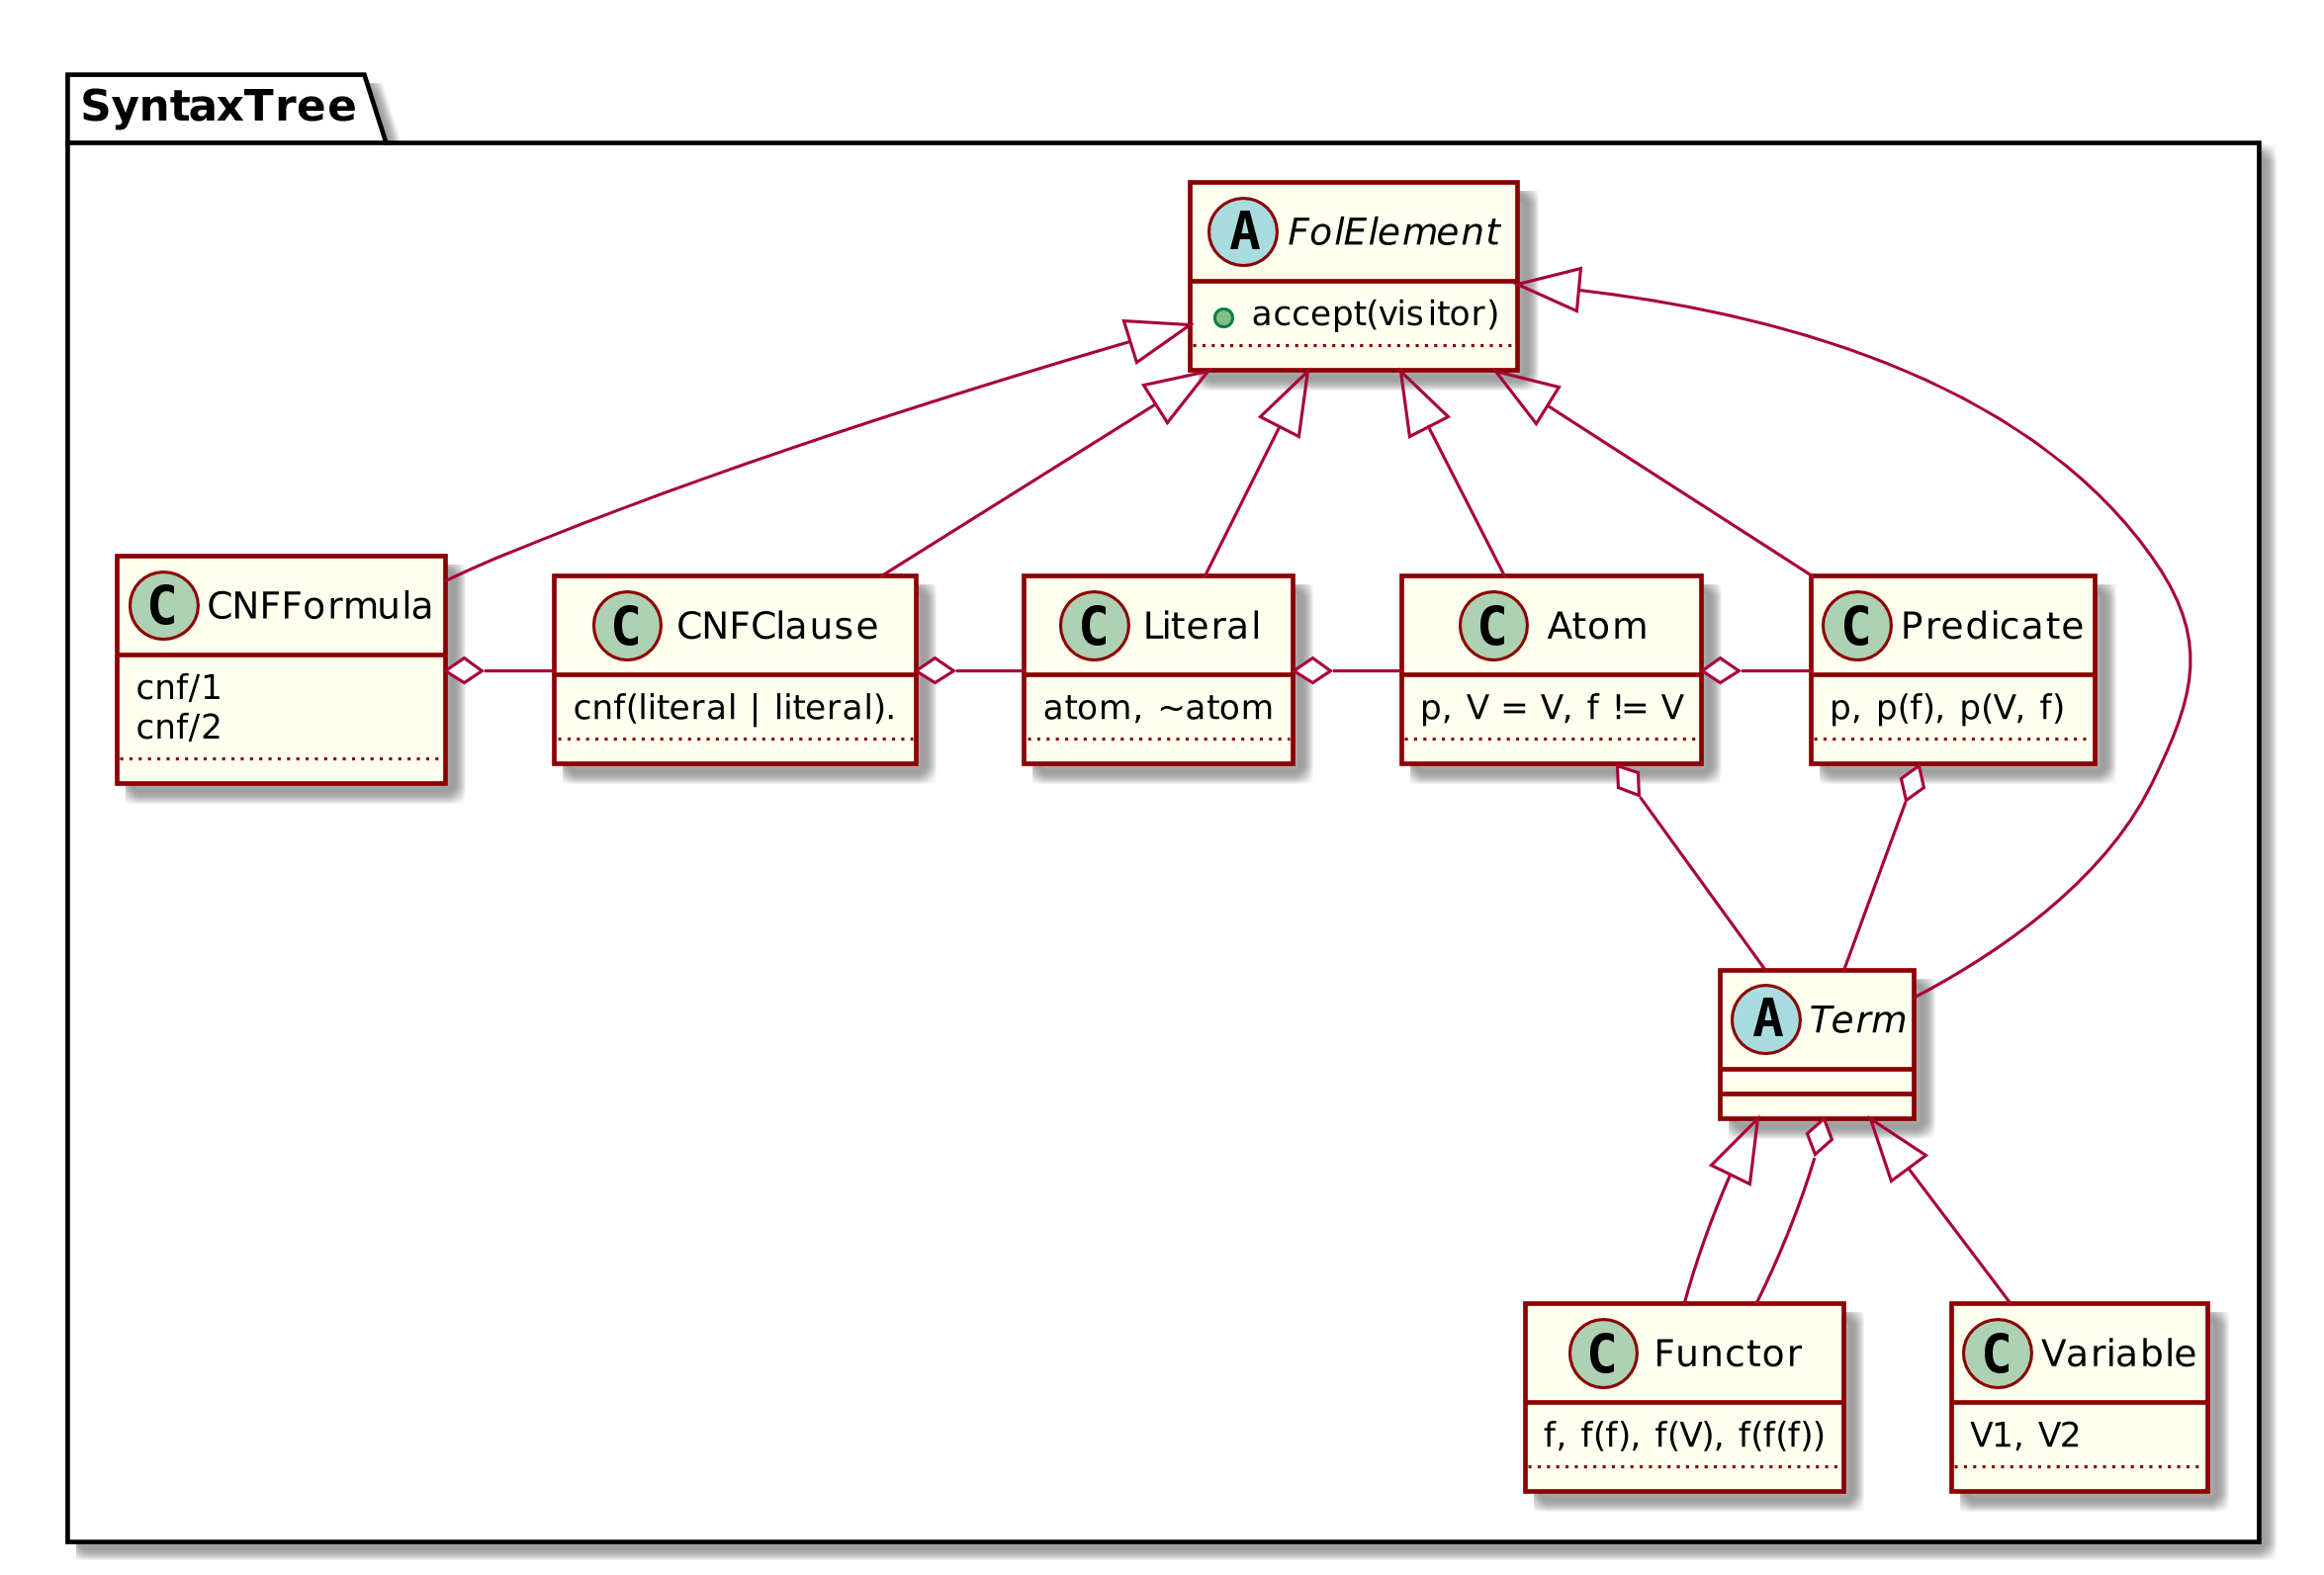
\includegraphics[width=\textwidth]{logic-formula-generator/fol/cnf_fol_elements.png}
  \caption{Class diagram for internal representation of first order logic elements}
\end{centering}
\end{figure}

\section{Generators}


\begin{figure}[H]
\begin{centering}
  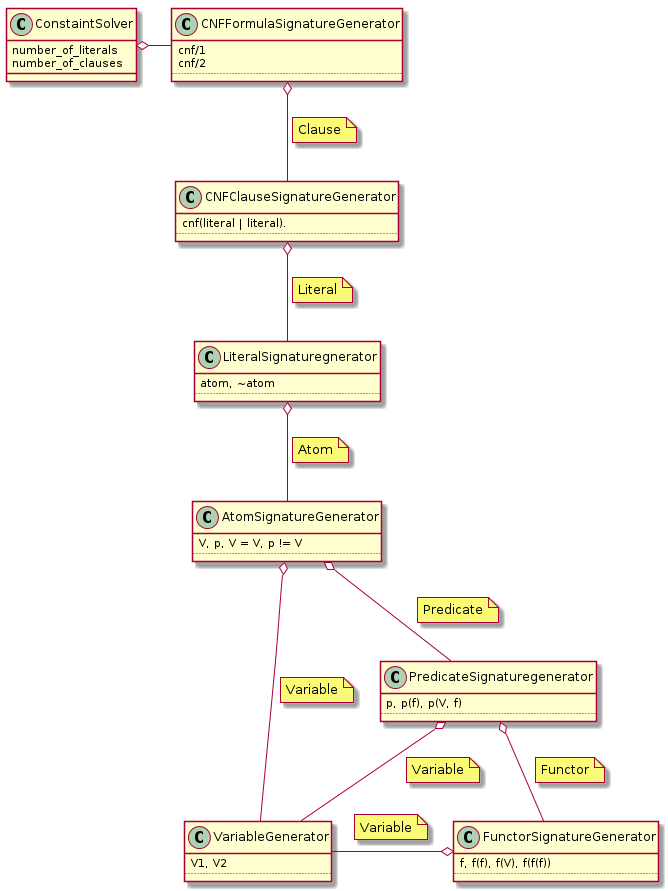
\includegraphics[width=0.7\textwidth]{logic-formula-generator/fol/cnf_signature_generators.png}
  \caption{Class diagram of generators in frst order logic}
\end{centering}
\end{figure}

\begin{figure}[H]
\begin{centering}
  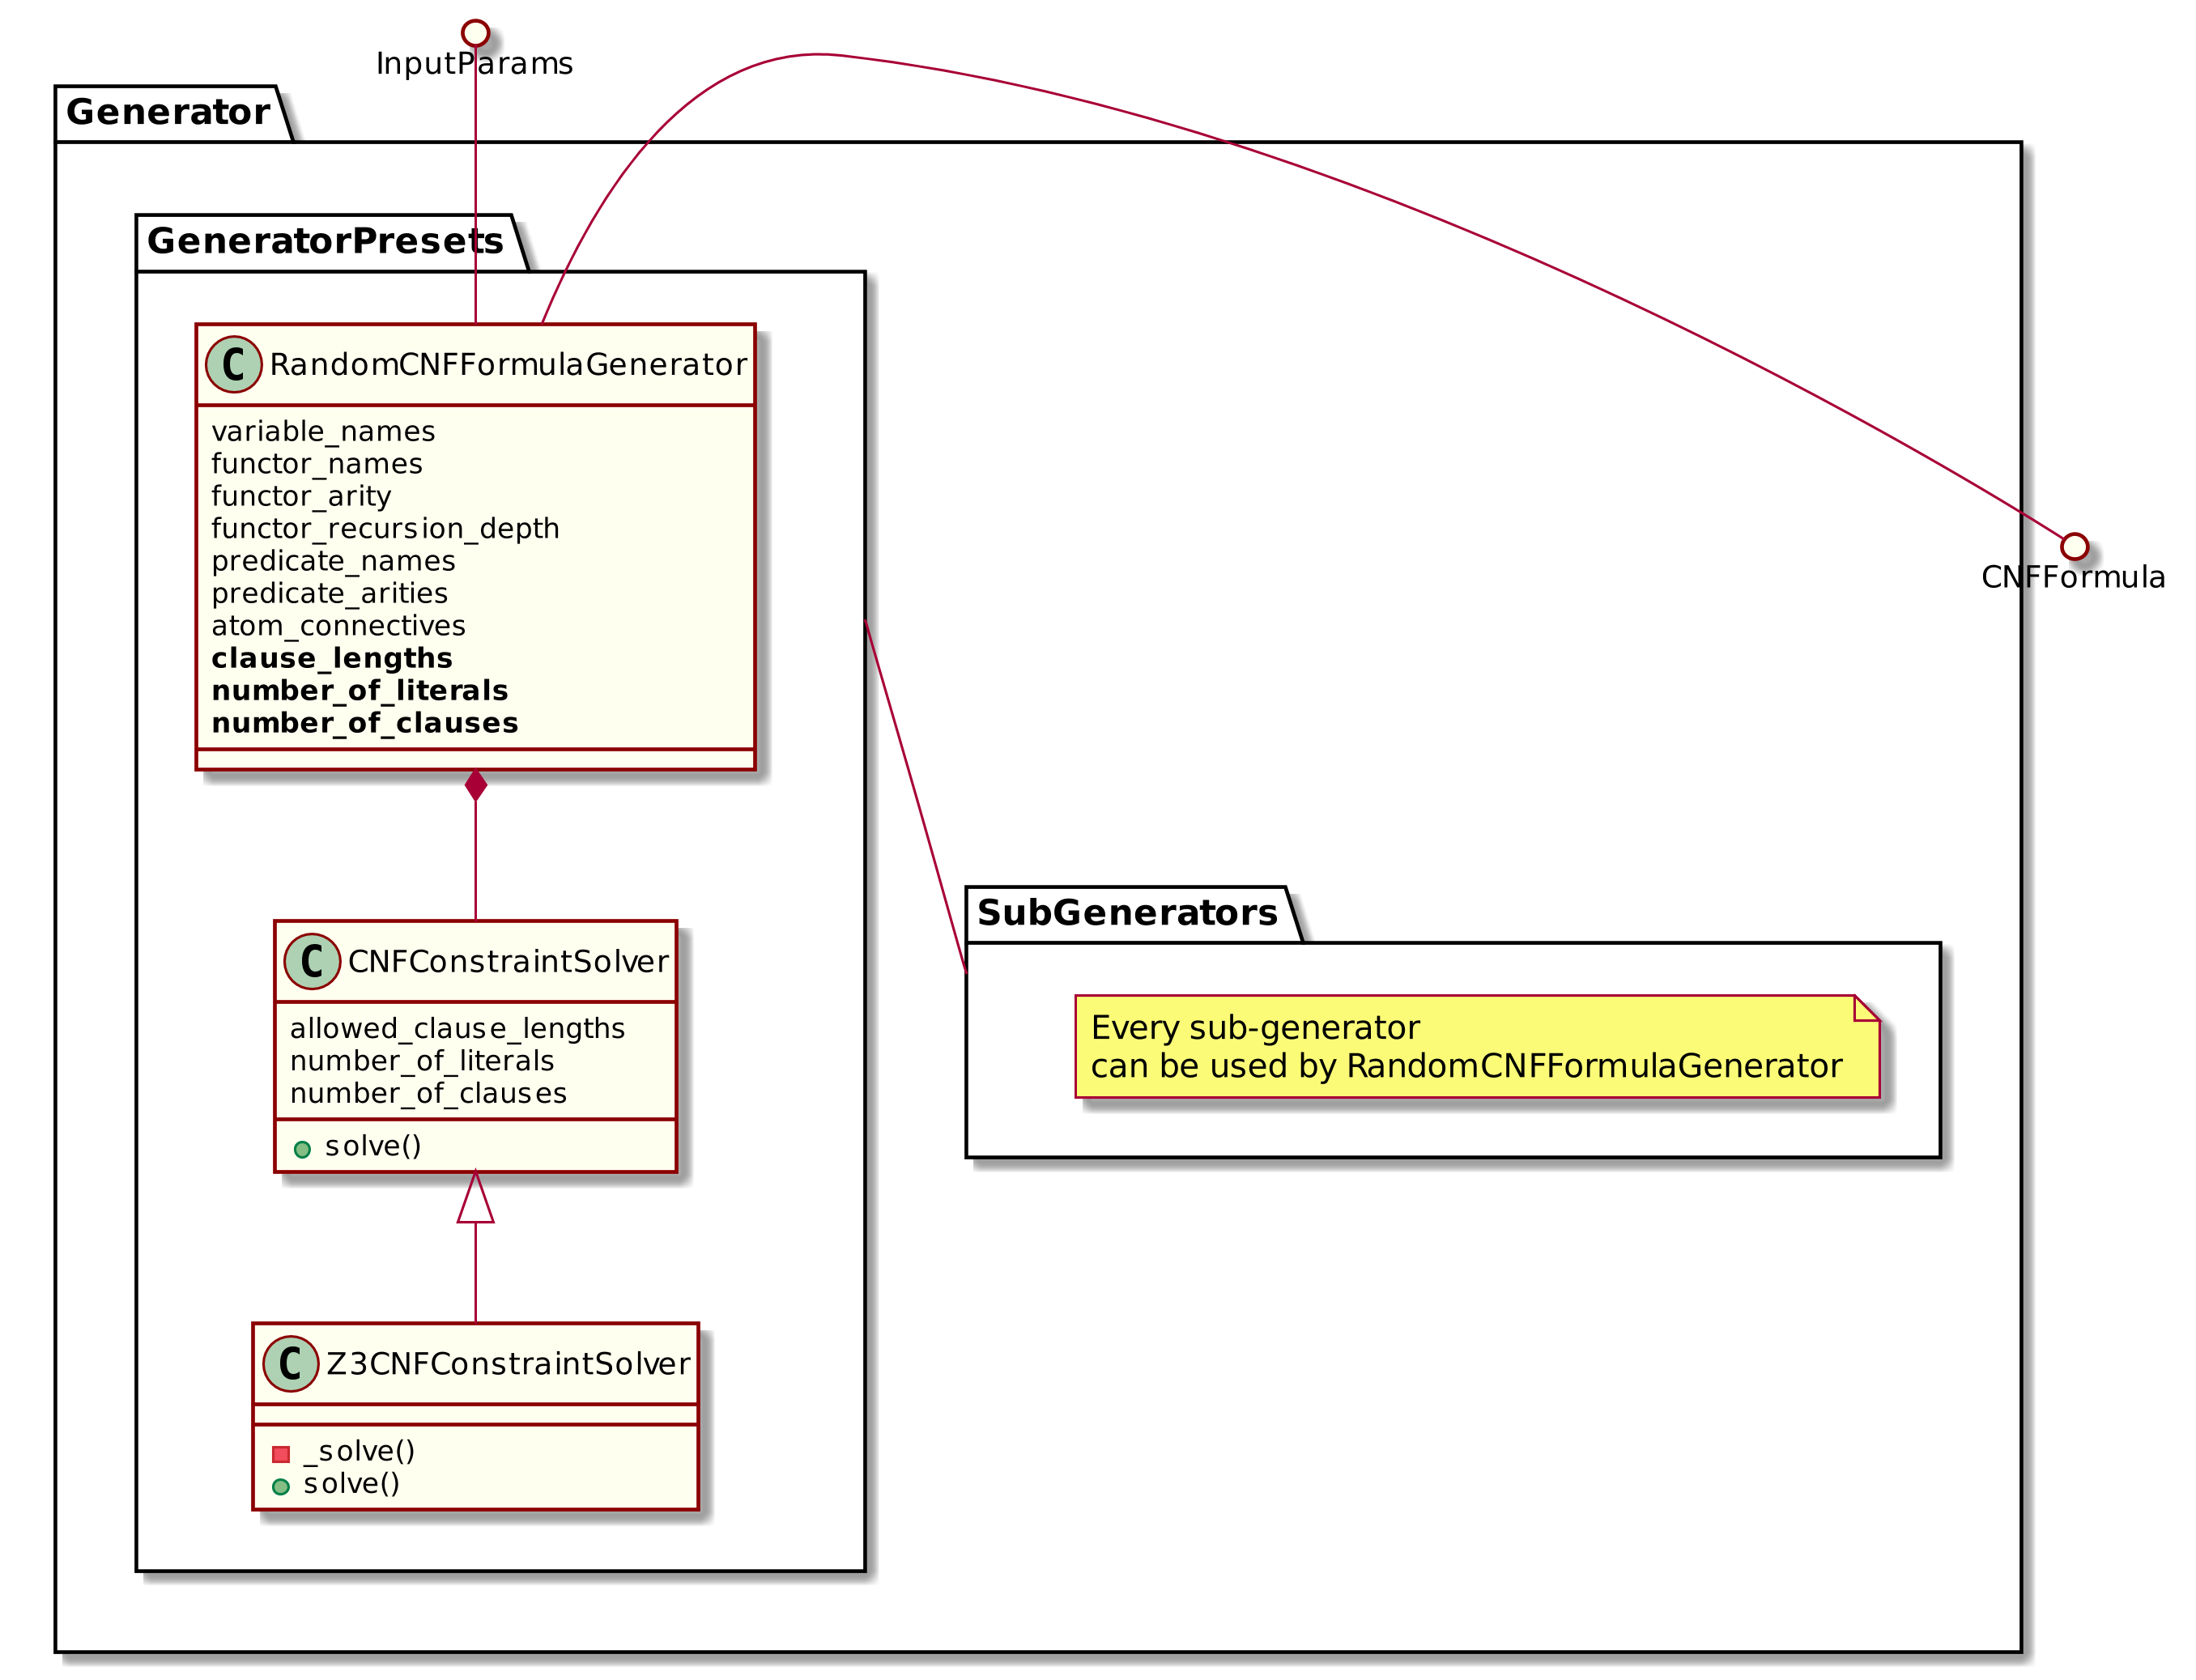
\includegraphics[width=0.7\textwidth]{logic-formula-generator/cnf_formula_generator.png}
  \caption{Class diagram of CNF forrmula generator}
\end{centering}
\end{figure}

\subsection{Functor}

Functor can contain variable or another functor.
Given that
$n$ is functor recursion depth,
$a$ is functor arity,
$f(n, a)$ number of functor signatures can be produced.

\begin{align}
	&f(n, a) =
	\begin{cases}
    a, \text{for } n = 0, \\
		a \sum_{i=n}^{i=1} \sum_{j=a}^{j=0} f(n-i,a-j) \\
	\end{cases}
\end{align}

Given that functor arity $a_f$ is in range $[a_{fmin}, a_{fmax}]$  and maximal recursion depth is $n_{max}$, $f(n_{max}, a_{fmin}, a_{fmax})$ number of functor signatures can be produced.

\begin{align}
  f(n_{max}, a_{fmin}, a_{fmax}) = \sum_{i=0}^{n_{max}} \sum_{j=a_{fmin}}^{a_{fmax}} f(i, j) \label{eq:functor}
\end{align}

\subsection{Predicates}

Predicates can contain functors or variables.
Given that $a_p$ is predicate arity, $P(a_p)$ number of predicate signatures can be produced.

\begin{align}
	P(a_p) &=
	\begin{cases}
		1, \text{for } a_p = 0 \\
		(f(n_{max}, a_{fmin}, a_{fmax}) + 1)^{a_p}, \\
	\end{cases}
\end{align}

Given that predicate arity $a_p$ is in range $[a_{pmin}, a_{pmax}]$, $p(a_{fmin}, a_{fmax})$ number of functor signatures can be produced.

\begin{align}
  p(a_{pmin}, a_{pmax}) = \sum_{i=a_{pmin}}^{a_{pmax}} p(i) \label{eq:predicate}
\end{align}

\subsection{Atoms}

Atom can contain only predicate. Single variable on its own is not an atom. Atom connects items with binary mathematical connective: $=$ or $!=$ or $\emptyset$ (no connective).
Given that atom $connective$, $A(connective)$ atom signatures can be produced.

\begin{align}
	A(connective) &= 
  \begin{cases}
    p(a_{pmin}, a_{pmax})^{2}, \text{for } connective \in \{'=', '!='\} \\
    p(a_{pmin}, a_{pmax}), \text{for } connective \in \{\emptyset\} \label{eq:atom}
  \end{cases}
\end{align}

% \subsection{Literals}
%
% Literal is atom or its negation.
%
% \begin{align}
  % L = A(AllowedConnectives) * 2 \label{eq:literal}
% \end{align}

\subsection{CNF Clause}

Clause $C$ can contain only atoms $A$. The order of atoms is irrelevant $C = \{a1, a2, \dots\}$

Given that 
clause length $l$ and 
set of unique atoms $A = \{a1, a2, \dots\}$, $\forall_{i,j \in L} i \neq j$
$C(a)$ clauses can be produced. Atoms can repeat.

\begin{align}
  C(l) = \binom{A + l - 1}{l}
\end{align}

Given that clause length $l$ is in range $[l_{min}, l_{max}]$

\begin{align}
  C(l_{min}, l_{max}) = \sum_{i=l_{min}}^{i=l_{max}} C(i) \label{eq:clause}
\end{align}

\subsection{CNF formulas}

Given that
formula contains $x$ clauses and
set of unique clauses $C = \{c1,c2, \dots\}$
$F$ formulas can be produced. Clauses can repeat.

\begin{align}
  &F_{cnf}(x) = C(l)^{x} \label{eq:cnfformula}
\end{align}

\chapter{Case study - generating random system properties}

One of the uses of random \gls{FOL} can be to generate random formula that represent system properties. That formula can be used as input for benchmark.

\section{Properties of computer systems}

System properties were first discussed in context of concurrency \cite{Lampert77} as a tool for formal verification multiprocess programs. One of first proposed properties were safety and liveness. These properties can apply to computer systems in general and be expressed in different formal systems.

\textbf{Liveness} \cite{Klimek99} is system property, that states, that something good will eventually happen.
Liveness formula guarantees that there is at least one case, where formula evaluates to true.

\textbf{Safety} \cite{Klimek99} is system property, that states, that something bad will never happens.
Safety formula must always be satisfied.

\subsection{Safety and liveness representation in logic systems}

In \gls{FOL} liveness and safety can be expressed as quantifiers, safety as universal quantifier and liveness as existential quantifier. Every \gls{FOL} can be converted to \gls{CNF}, so system properties can be also represented in \gls{CNF}, if needed. It can be done for example with otter algorithm \cite{McC-Otter-URL} or skolemisation.

In \gls{FOL} system properties could look like (first is example with quantifiers, followed by CNF equivalent)\footnote{removing quantiviers from first order logic can be automated with TPTP utility using TPTP2X utility, option \mintinline{text}{-t clausify:quaife} \ref{sub:AdditionalToolsInTPTPLibrary} }:
\begin{itemize}
  \item Safety formula: $\forall_X p(X) \equiv p(A)$
  \item Safety formula: $\forall_X p(X, X) \equiv p(A, B)$
  \item Liveness formula: $\exists_X p(X) \lor \equiv p1(f1)$
  \item Liveness formula: $\exists_X p(X, X) \equiv p(f1, f2)$
\end{itemize}

The combinations of quantifiers (that correspond to combinations of liveness and safety properties) are not discussed in this thesis. For example (first is example with quantifiers, followed by CNF equivalent):
\begin{itemize}
\item $\exists_Y \forall_X p(X, Y) \equiv p(f1, A)$
\item $\forall_X \exists_Y p(X, Y) \equiv p(A,f1(A)) $
\end{itemize}

Example of real life problem expressed in safety and liveness formulas is collisionless lights on crossroad.

\noindent
Problem: cars want to drive through crossroad.

\noindent
Safety property: only one light can be green.

\noindent
Liveness property: every light should eventually turn green.

\section{Generating dataset}

The goal is to generate liveness and safety clauses, but do not mix them. In order to achieve that, class $PredicateGenerator$ needs to be modified to yield either formulas with all variables (safety) or formulas with 0-arity functor (liveness). To achieve that $PredicateGenerator$ was subclassed and used to create alternative version of $CNFFormulaGenerator$.

\begin{figure}[H]
\begin{centering}
  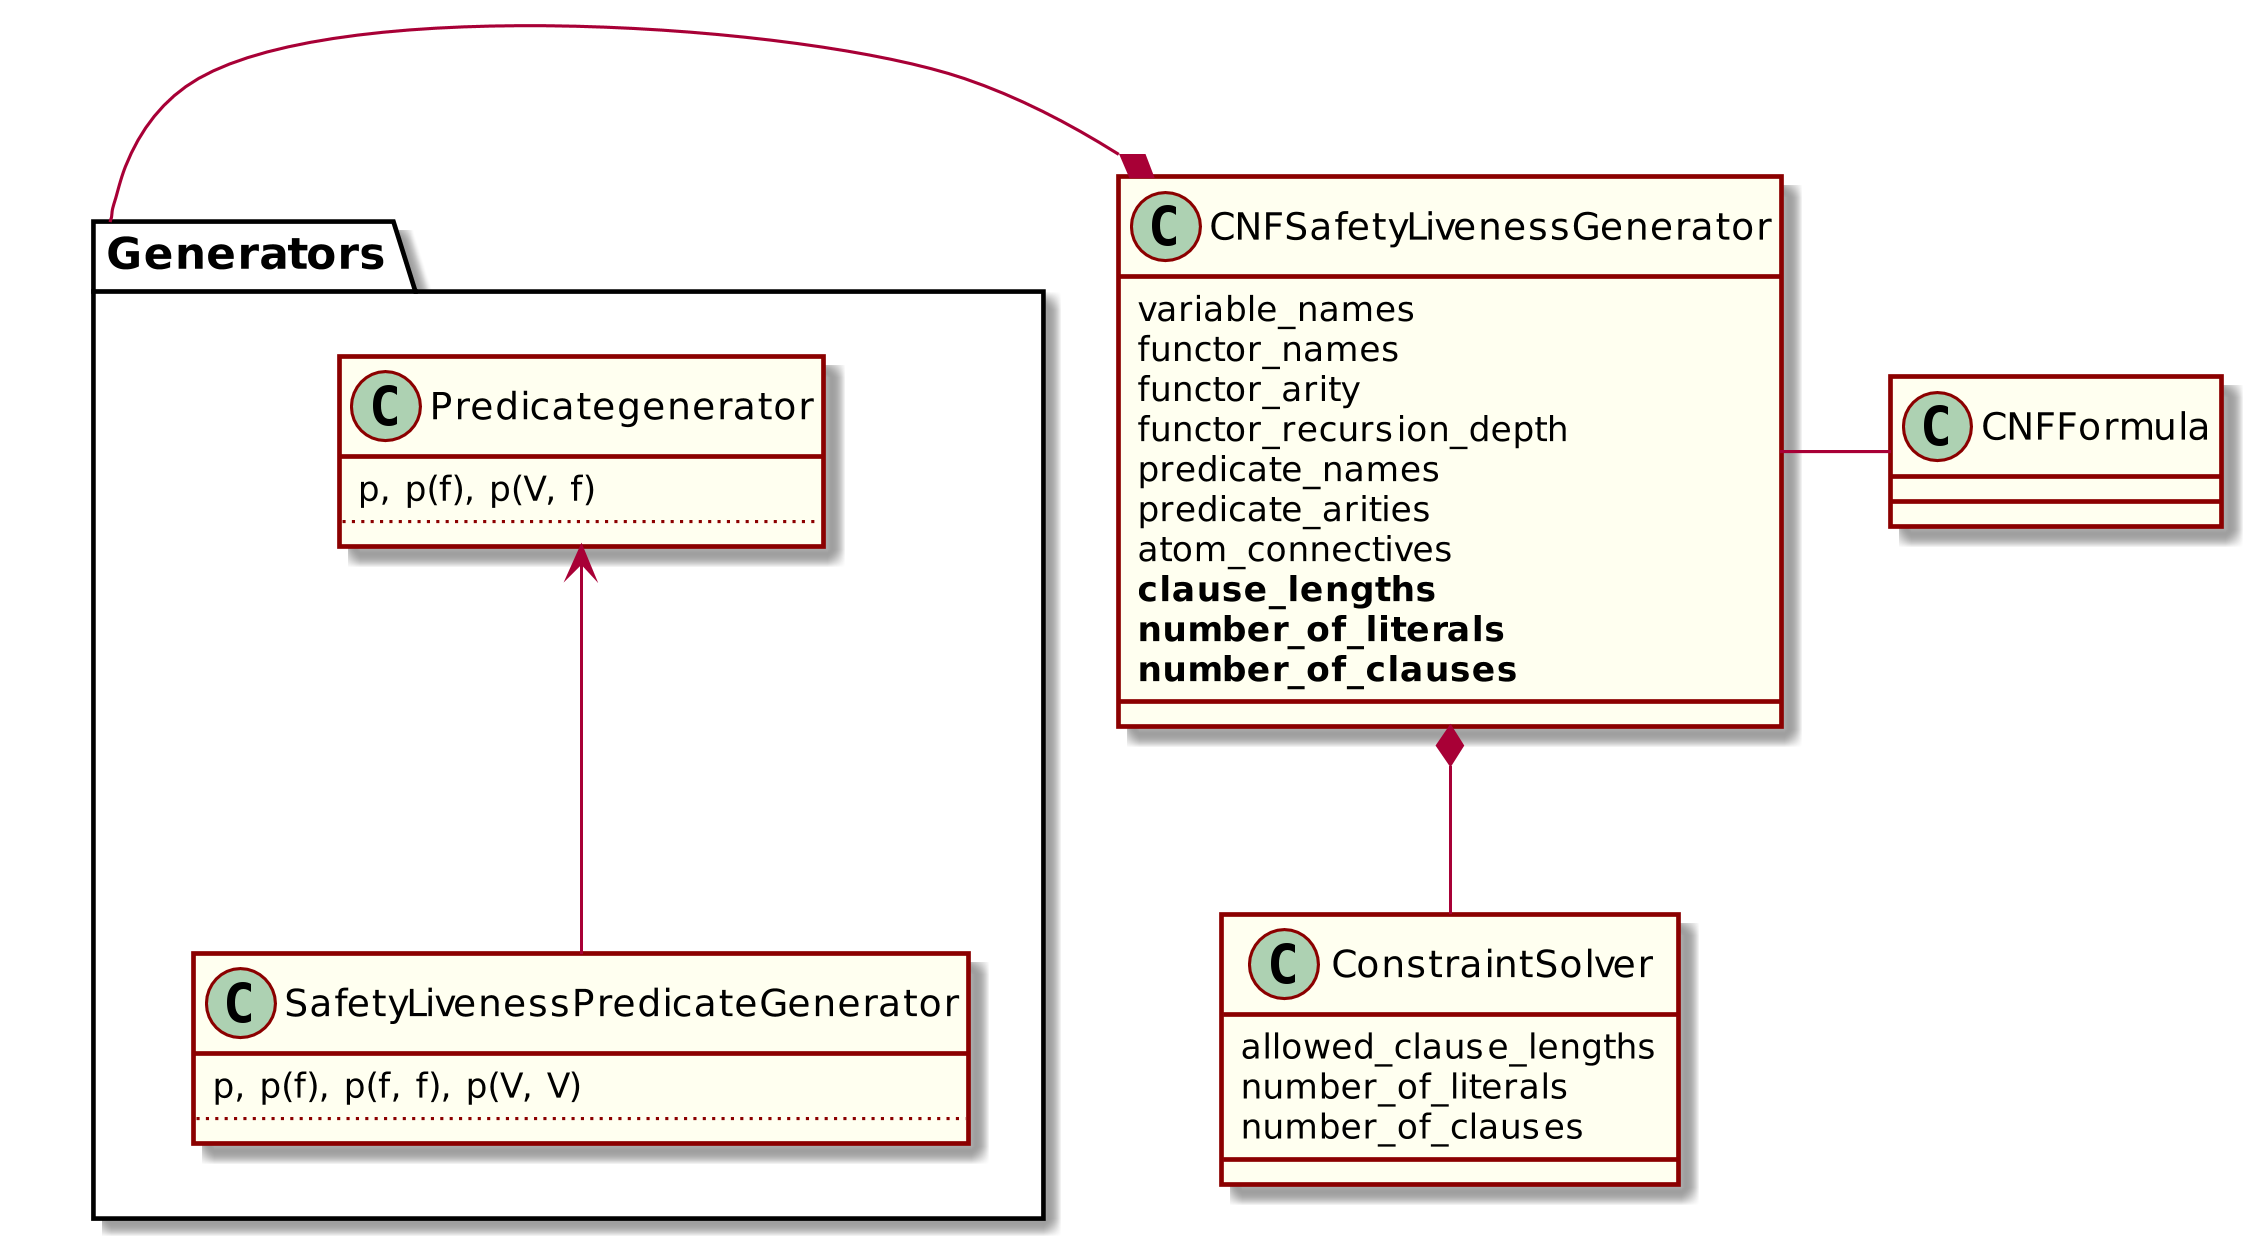
\includegraphics[width=\textwidth]{logic-formula-generator/fol/safety_liveness_predicate_generator.png}
  \caption{Subclassed PredicateGenerator mimics safety and liveness formulas}
\end{centering}
\end{figure}

In this study the impact of ratio of number of atoms to number of clauses will be presented.
Formulas with 1000 atoms and 100, 200, 300, 400, 500 clauses were generated, 50 for each combination, 250 in total. 50 formulas is rather small sample to reason about, but it was chosen because of time and hardware limitations. Number of atoms and number of clauses can vary within 5\%, although solver tends to yield small numbers first in general. The rest of parameters for formulas is shown in listing \ref{lis:CNFSafetyLivenesSnippet}.

\section{Results}

Formulas were generated and were benchmarked against solvers Prover9 and SPASS. Results are shown in pictures \ref{pic:SPASSProverNumberOfClauses} and \ref{pic:SPASSProverMemory}. Maximum execution time of single formula was trimmed at 300 seconds. 

First thing worth noting is SPASS solver is capable of solving much more formulas than Prover9. SPASS uses somewhat constant memory whereas Prover9 requires more memory the longer it runs.

It can be said that formulas with ratio atoms to clauses below 4 can be considered easy, as all of them were solved by both solvers.

\begin{listing}[ht]
  \caption{Snippet for generating dataset of safety and liveness formulas}
  \label{lis:CNFSafetyLivenesSnippet}
\begin{minted}{python}
gen = CNFSafetyLivenessGenerator(
    variable_names={f'V{i}' for i in range(10)},
    functor_names={f'f{i}' for i in range(20)}, functor_arity={0},
    functor_recursion_depth=0,
    predicate_names={f'p{i}' for i in range(20)}, predicate_arities={i for i in range(5)},
    atom_connectives={''},
    clause_lengths={i for i in range(2, 11)},
    number_of_clauses=IntegerRange.from_relative(number_of_clauses, threshold),
    number_of_literals=IntegerRange.from_relative(number_of_literals, threshold),
    literal_negation_chance=0.1,
)
\end{minted}
\end{listing}

\begin{listing}[ht]
  \caption{Example of generated formula (limited)}
\begin{tptpcode}
% ----------------------------------------------------------------------------
% File      : 0.p 
% Syntax    : Number of clauses     :   95 ( 95 non-Horn;   0 unit;   - RR)
%             Number of atoms       :  950 (  0 equality)
%             Maximal clause size   :   10 ( 10 average)
%             Number of predicates  :   20 (206 propositional; 0-4 arity)
%             Number of functors    :   20 (940 constant;   0 arity)
%             Number of variables   :  943 (327 singleton)
%             Maximal term depth    :    0 (  - average)
% 
% ----------------------------------------------------------------------------
cnf(name,axiom,p4(V6)|p10(V1, V4, V9)|~p7|p17|p1(V4, V3, V9)|p7|p17|p1(f11, f11, f5)|p7|~p0(f2)).
cnf(name,axiom,p2(V7, V9)|p4(f19)|p2(f8, f5)|p10(f7, f8, f8)|p12|p6(V2, V6)|p14(f8, f16, f9, f16)|p3(f14, f3, f14, f18)|p11(V3, V9)|p12).
...
\end{tptpcode}
\end{listing}

\begin{figure}[ht]
\centering
  \begin{subfigure}{0.9\textwidth}
\centering
  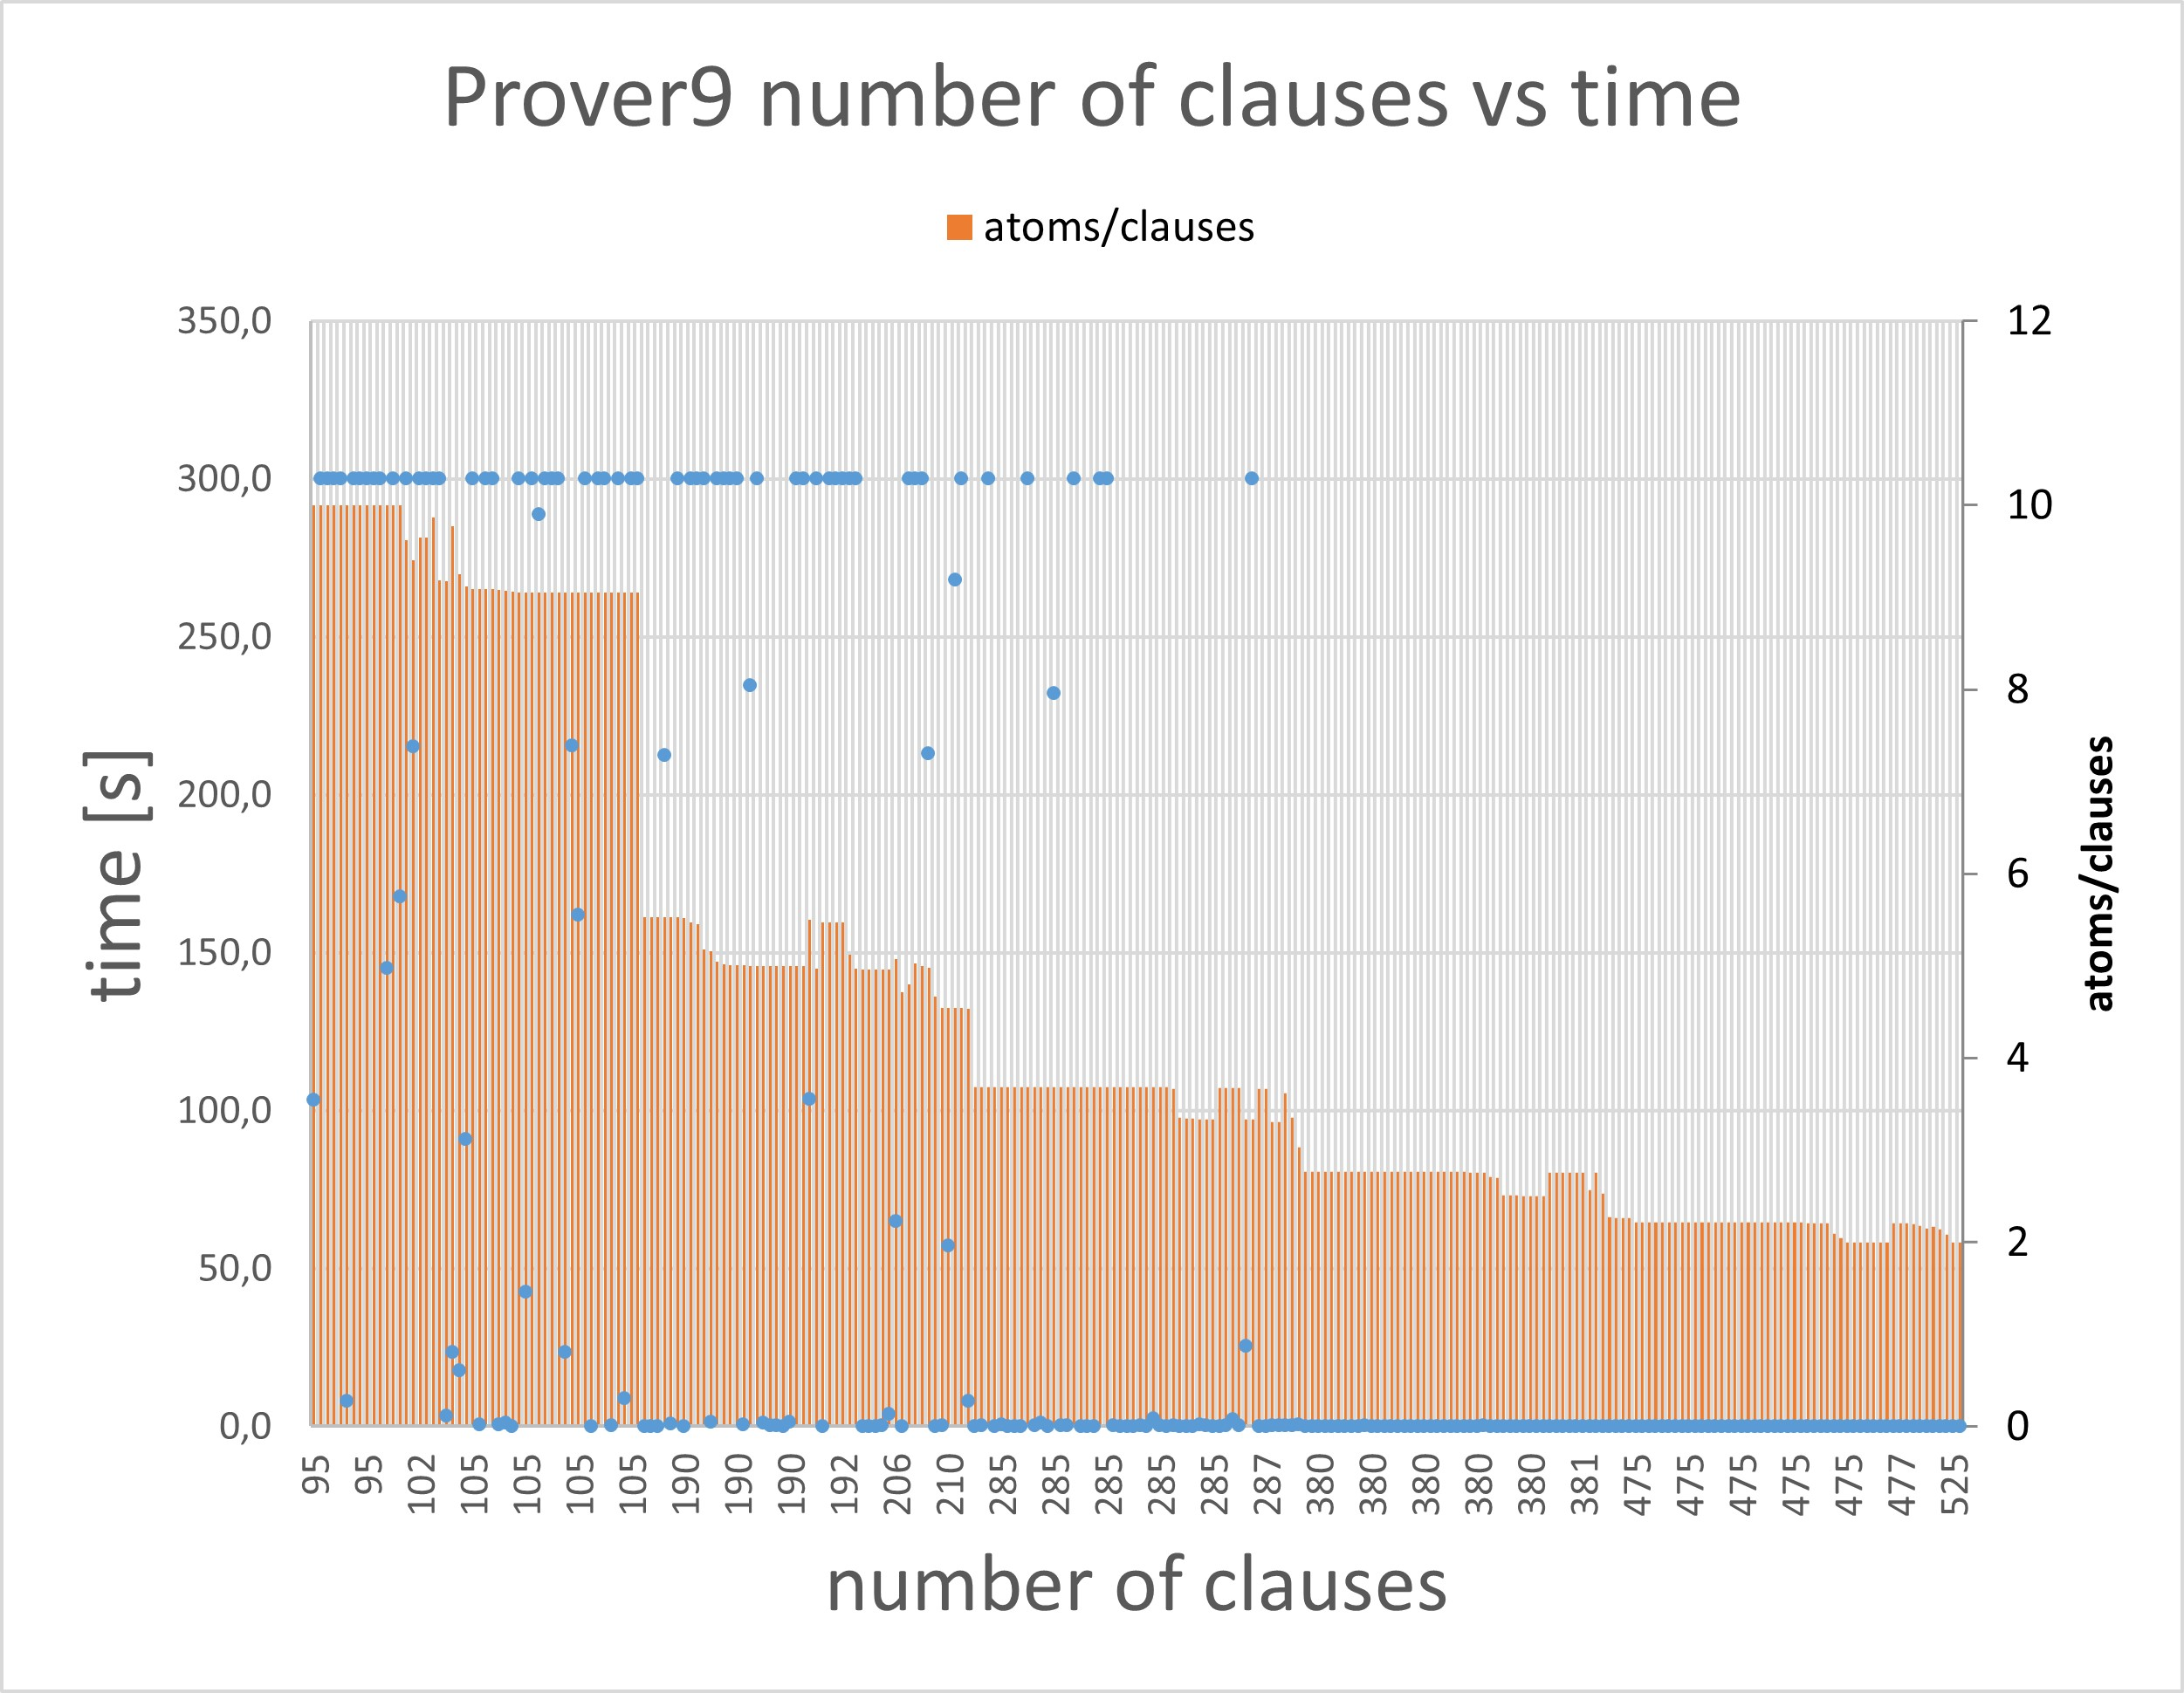
\includegraphics[width=\textwidth]{logic-formula-generator/dataset_analysis/cnf charts/01 Prover9 number of clauses vs time.jpg}
  \label{pic:benchmark_results}
  \end{subfigure}

  \begin{subfigure}{\textwidth}
\centering
  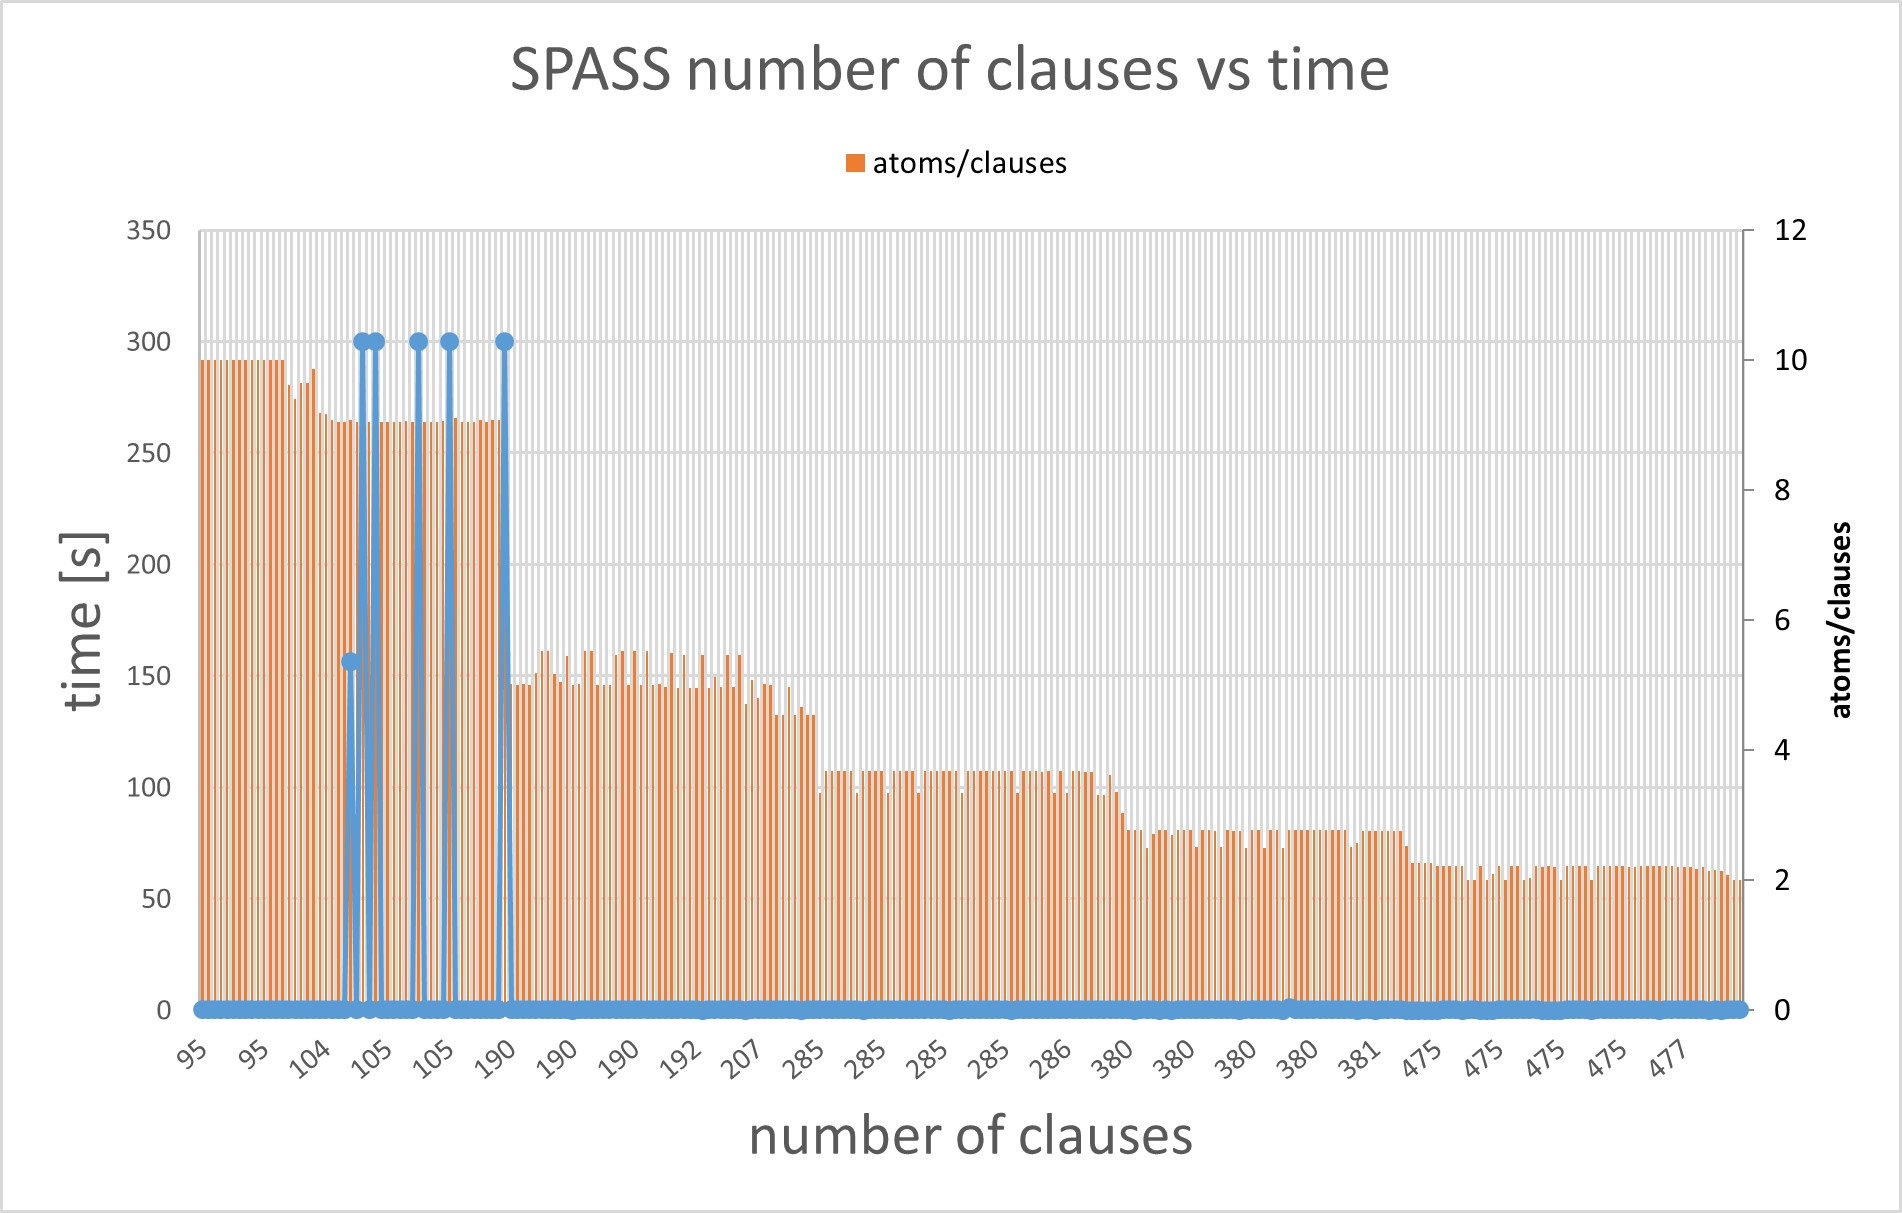
\includegraphics[width=\textwidth]{logic-formula-generator/dataset_analysis/cnf charts/11 SPASS number of clauses vs time.jpg}
  \end{subfigure}
  \caption{On left axis time of execution is presented (300s is max), marked with blue. On right axis ratio clauses to atoms is presented. Ratio 2 means there are 2 atoms for each clause}
  \label{pic:SPASSProverNumberOfClauses}
\end{figure}

\begin{figure}[ht]
\centering
  \begin{subfigure}{0.85\textwidth}
\centering
  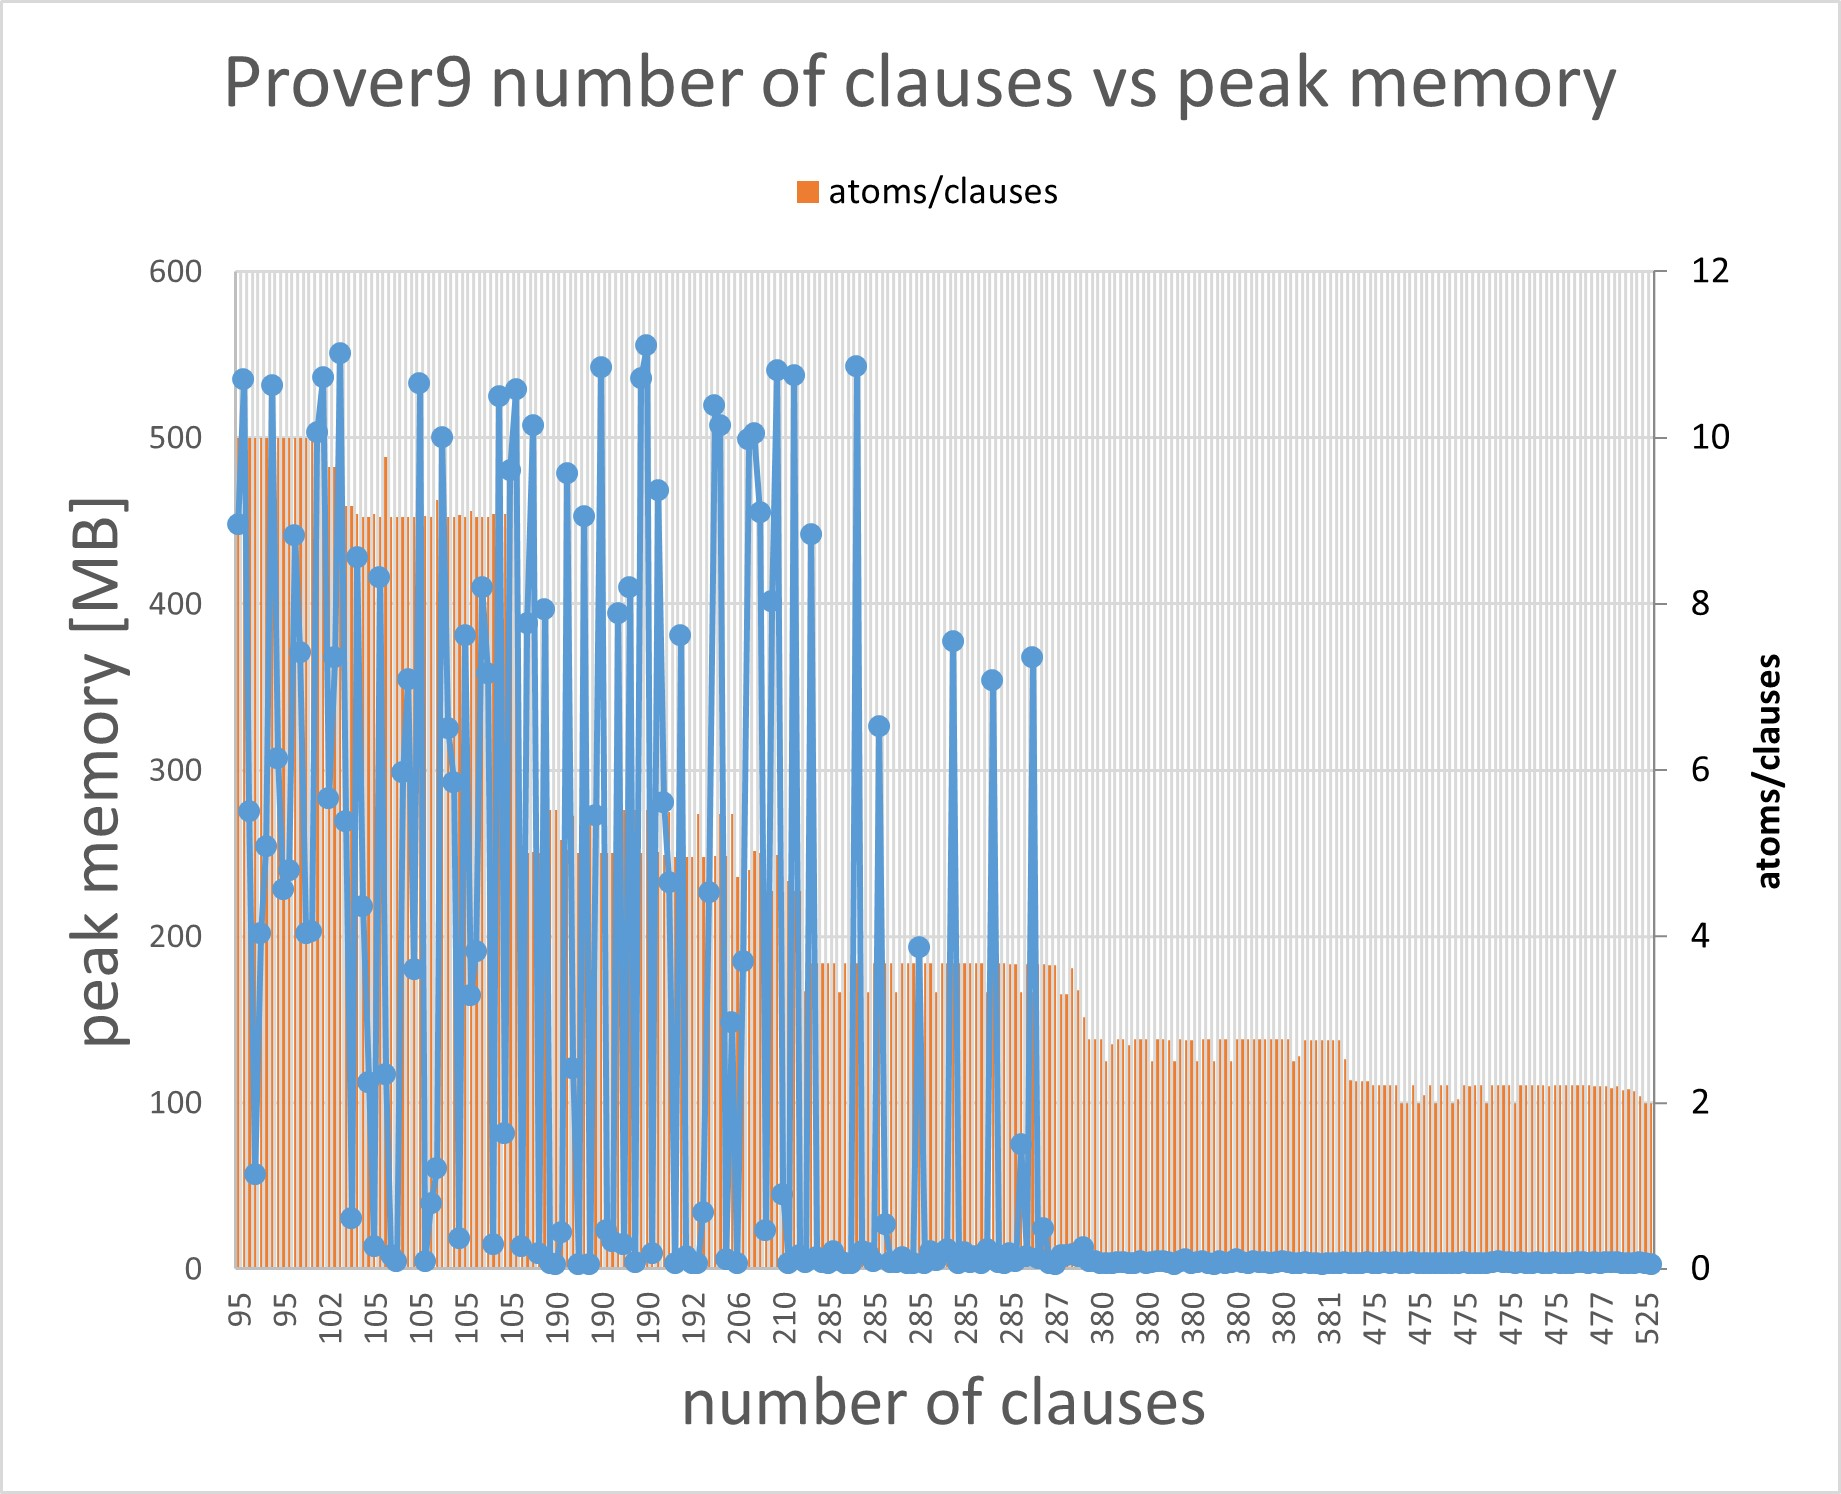
\includegraphics[width=\textwidth]{logic-formula-generator/dataset_analysis/cnf charts/02 Prover9 number of clauses vs peak memory.jpg}
  \label{pic:benchmark_results}
  \end{subfigure}

  \begin{subfigure}{\textwidth}
\centering
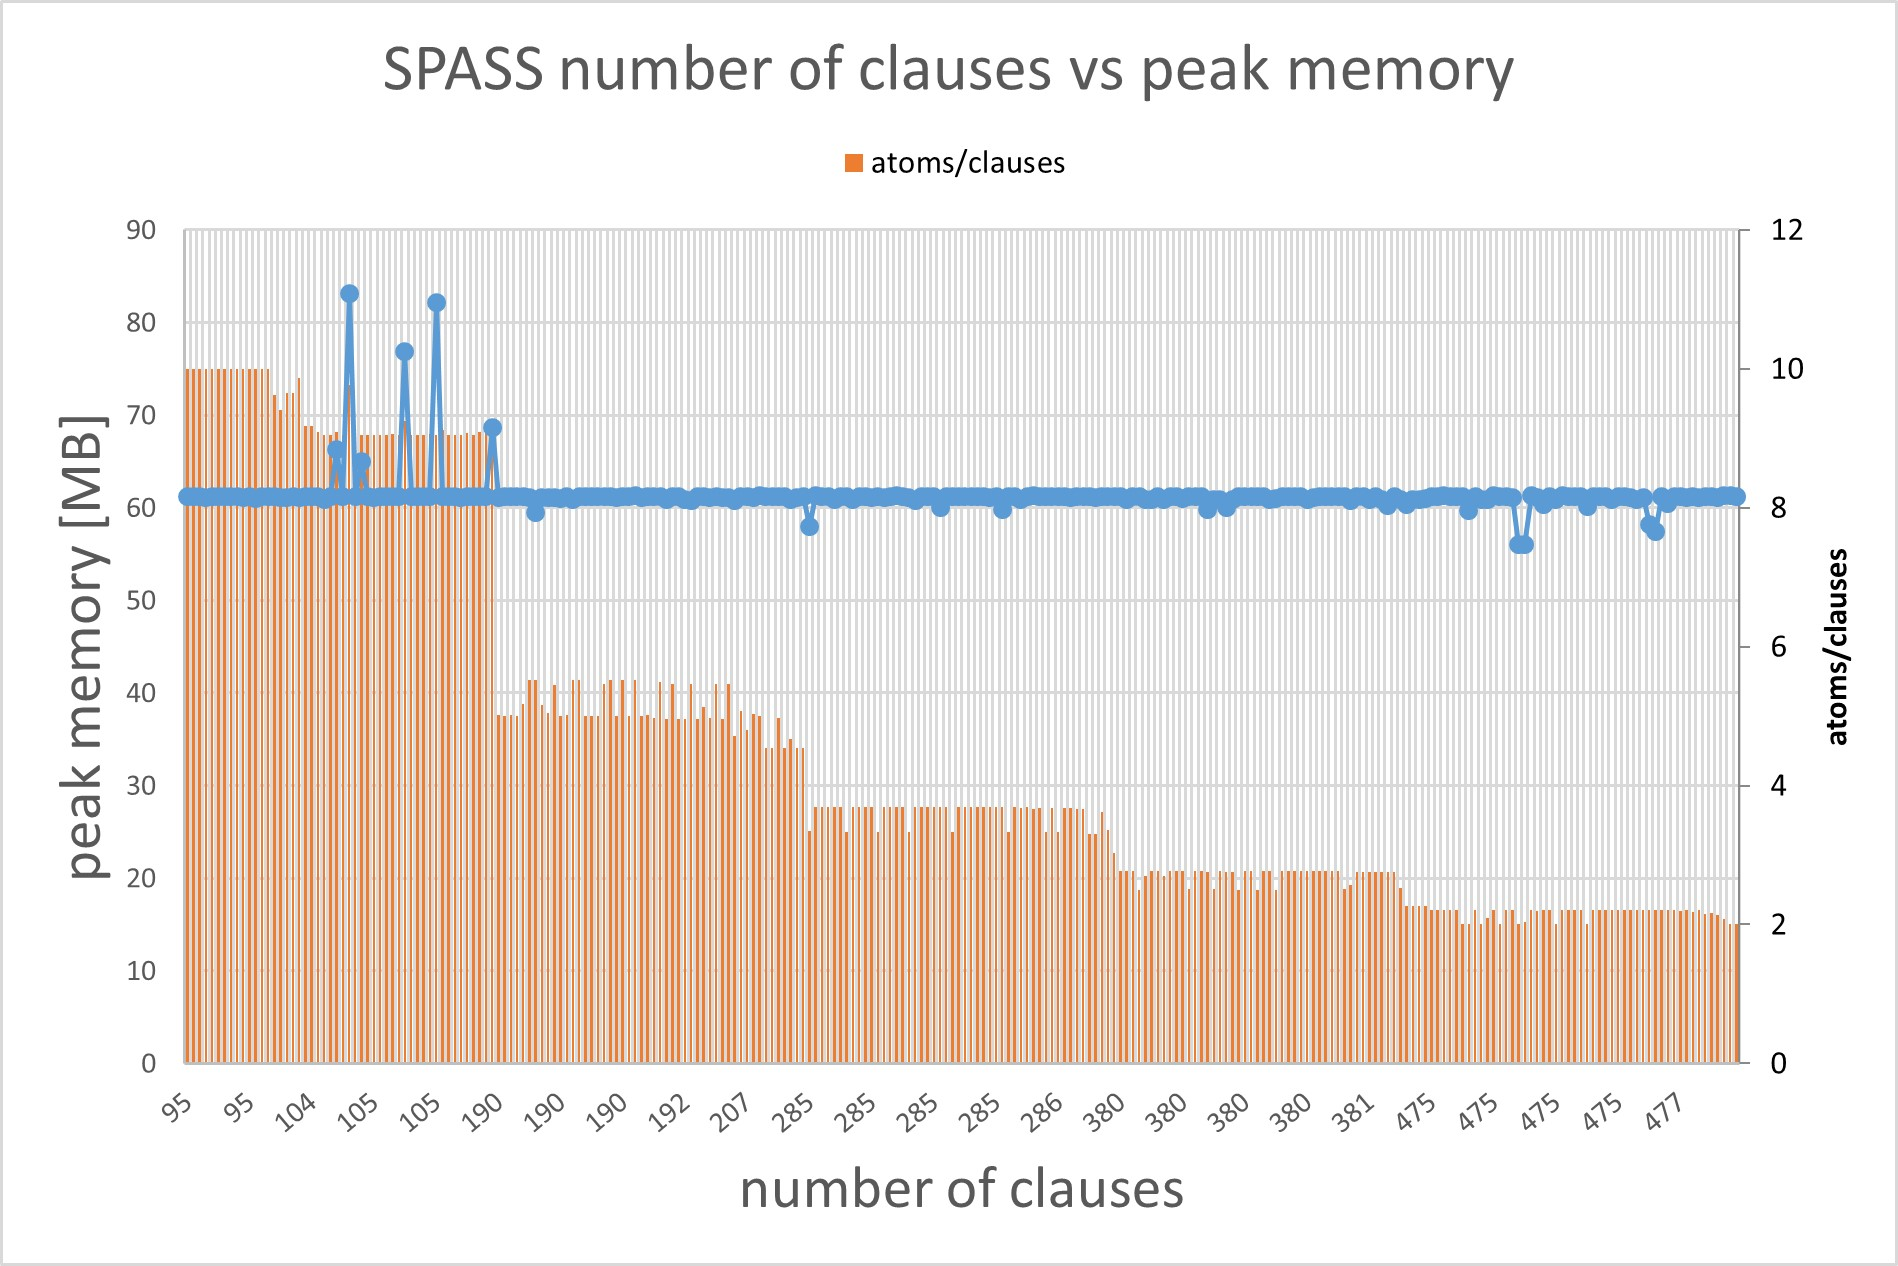
\includegraphics[width=\textwidth]{logic-formula-generator/dataset_analysis/cnf charts/12 SPASS number of clauses vs peak memory.jpg}
  \end{subfigure}
  \caption{On left axis peak RAM memory is presented, marked with blue. On right axis ratio clauses to atoms is presented. Ratio 2 means there are 2 atoms for each clause}
  \label{pic:SPASSProverMemory}
\end{figure}


\chapter{Conclusion}

In this thesis a base for random first order logic formula generator has been presented. The generator can be easily extended for user specific needs. For example user can add arbitrary rule that elements must follow during generation, more output format can be added. The biggest challenge in described algorithm is time and memory complexity. Described approach takes into consideration fact, that there are finite number formulas within user given restrictions - if user requests too many formulas, they will start to repeat what may not be desirable. Solving user constrains with Z3 solver is NP problem and generating combinations and permutations in \textit{random} order requires additional memory.

Alternative approach to using SMT solver would be to take locally optimal decisions and introduce some randomness when taking those decisions. This approach would create arguably "more" random result but introduces number of drawbacks:

\begin{itemize}
  \item taking many local decisions may not be faster than taking one global - that requires in depth analysis,
  \item this is non deterministic approach - some possible variants of formula might never/rarely be reached,
  \item there is no way of detecting duplicate formulas without storing them.
\end{itemize}

The future development of presented generator would allow to generate formulas in different normal forms, more readable suggestions for constrains errors and ability to auto correct user constraints errors.



% itd.
% \appendix
% \include{dodatekA}
% \include{dodatekB}
% itd.

\printglossary

\printbibliography

\end{document}
